\documentclass[11pt]{article}

\usepackage[utf8]{inputenc}
\usepackage{graphics}
\usepackage{graphicx}
\usepackage[margin=2.8cm]{geometry}
\usepackage{placeins}

\usepackage{titlesec}
\setlength{\parindent}{0pt}
\setlength{\parskip}{1em}
\titlespacing{\section}{0pt}{\parskip}{-\parskip}
\titlespacing{\subsection}{0pt}{\parskip}{-\parskip}

\usepackage{hyperref}
\hypersetup{
    colorlinks   = true,
    urlcolor     = blue,
    linkcolor    = black
}

\title{{\large MSE491 - Application of Machine Learning in Mechatronic Systems} \\ Project Proposal: \\ Vessel Targeting System for Automated Gantry Robot}
\author{Group 24 \\ Liam Akkerman - 301286906 \\ Aidan Hunter - 301279938}

\begin{document}
    \maketitle
    \newpage

    \section{Summary}
        There is an industrial production line which centres around jars. A step is that jars are washed by being placed in a washing tray and passed through a commercial dishwasher. After exiting the dishwasher, the jars have changed position. To allow for automation, robotics may be added to unload from the clean trays. The robotics require require precise coordinates to function. Because the jars are not in a constant position, a vision system may be implemented to accurately determine these coordinates for each jar.

        \textbf{Data}: Numerous 2d images of jars in trays. Top-down perspective.

        \textbf{Data Collection}: Manually arranging jars in a tray randomly and taking a photo with a Raspberry Pi camera from a consistent perspective. It will be done by us.

        \textbf{Features}: An image converted to a \( (m,1) \) vector of features.

        \textbf{Target}: Either a list of coordinates of all jars in a given image, or the coordinates of the jar closest to the exit.

    \section{Introduction}
        Industrial automation is an industry which is very applicable for mechatronic systems. Semi-automated systems utilize a mix of human and robot labour to preform a task. Though robots will preform a task nearly identical each time, a human worker will not. To rectify this, humans may be trained to be more uniform or a subsystem may be employed to account for this variance. Machine learning is an ideal tool for working with an inconsistent states.

        A group member, Liam, works with a certain company doing industrial automation. The company does micropropagation, a plant cloning technique, using glass jars as vessels. The vessels must be washed after use. Liam has conducted projects automating these processes. They currently are semi-automated and require a human technician to operate.

    \section{Problem Description}
        A large portion of the work required for the technician is both moving emptied jars from a conveyor belt into a dishwashing tray and washed jars from a tray onto a conveyor belt. A subsystem which moves jars into trays could have hard coded positions. After the trays come through the dishwasher, the jars do not have consistent positions. 

        Using computer vision, a computer such as a Raspberry Pi could ascertain the positions of the jars in the tray. This would be a classification problem. In essence, it is finding the centre of circles from a still image. This project will be the creation of the vision system. Presumed implementation details may be found in section~\ref{sec:imp}.

        This would be in conjunction with a cancelled project for the company. The project involved a gantry robot using an internal gripper to move jars, an example is shown in figure~\ref{fig:gantry}. The gripper would be either pneumatic powered or servos.

        \begin{figure}[ht]
            \centering
            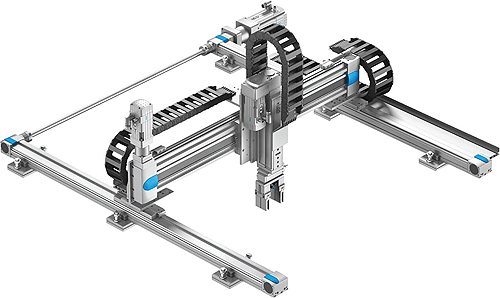
\includegraphics[height=5.5cm]{gantry.jpg}
            \caption{Festo 3d Gantry Robot}\label{fig:gantry}
        \end{figure}

    \FloatBarrier
    \section{Materials Required}
        \subsection{Commercial Dishwashing Tray}
            Vessels are to be loaded and unloaded from a commercial dishwashing tray. They are a standard size as a 19-3/4" by 19-3/4" square. A tray may be collected from Liam's work. One is sufficient. 

            \begin{figure}[ht]
                \centering
                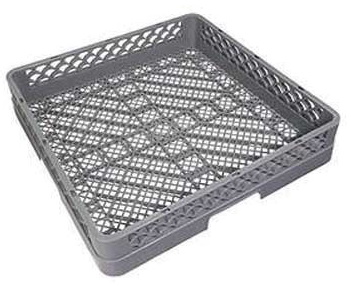
\includegraphics[height=7cm]{tray.jpg}
                \caption{Commercial Dishwashing Tray}\label{fig:tray}
            \end{figure}

        \FloatBarrier
        \subsection{Glass Jar}
            The jars used are 80mm diameter and 110mm tall. 26 jars are required which is the maximum amount of jars that fit in a tray. The jars may be collected from Liam's work. The jar shown in figure~\ref{fig:jar} is not the exact jar but close.

            \begin{figure}[ht]
                \centering
                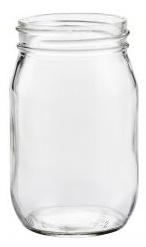
\includegraphics[height=7.5cm]{jar.jpg}
                \caption{Glass Jar}\label{fig:jar}
            \end{figure}

        \FloatBarrier
        \subsection{Camera}
            This may be an official Raspberry Pi camera or simply a USB web-camera. The only Requirement is sufficient resolution and field of view. A specific camera has not been chosen yet.

            \begin{figure}[ht]
                \centering
                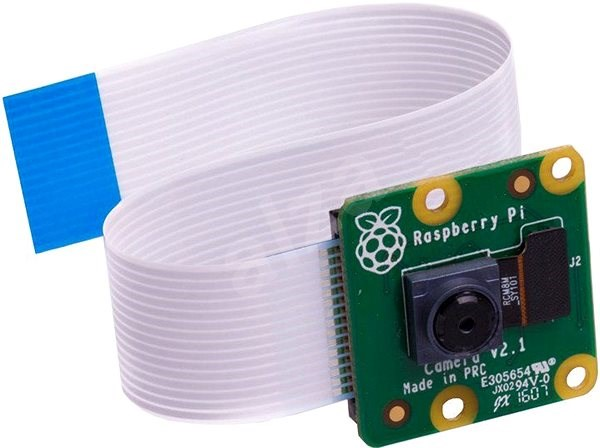
\includegraphics[height=5cm]{camera.jpg}
                \caption{Raspberry Pi Camera}\label{fig:camera}
            \end{figure}

    \section{Implementation}\label{sec:imp}
        \subsection{Hardware}
            The camera may be mounted directly above where the full trays are placed. This will provide a top-down view of the jars. Fiducial markers may be required for calibration purposes. 

            A Raspberry Pi Zero should provide sufficient computational power for the vision system but would not be capable of also running the control for the gantry robot. Raspberry Pis are known for poor precise real-time performance and can only overcome it with more computation. Only the vision system is within the scope of this project thus the Raspberry Pi Zero will suffice.

            If necessary, brightly coloured bands may be added to the jars to better distinguish them from the tray.

        \subsection{Software}
            The classification algorithm will need to experimented with thus no definitive algorithm may be chosen at this time.

            The input data will be an image of the tray and jars. This will need to be parameterized into features. More research will need to happen for a better understanding of this process. The target will be either a list of X Y coordinates of each jar, or just the coordinates of the closest remaining jar to the exit.

            A large pool of data may be collected by moving around jars in the tray and taking a picture. Rotating the image may provide an easy way to quadruple the dataset. Different amounts of jars and different colour trays may be used for added robustness.

            In the original project, the coordinates would be used the generate g-code on the fly to control the gantry robot.

            The camera may be controlled or integrated using tools such as \href{https://github.com/silvanmelchior/RPi_Cam_Web_Interface}{RPi-Cam-Web-Interface} or \href{https://github.com/waveform80/picamera}{picamera}. This would allow the video feed to be imported to python and monitored via a web interface.

\end{document}
